% ====================================================================
% v7-09.tex — graphite anode dQ/dV ICA theory Chapter 1
% Source spine: Anode_Fit_v11_final.py and v11_flowchart.md
% ====================================================================
\documentclass[11pt,a4paper]{article}
\usepackage[margin=22mm]{geometry}
\usepackage{kotex}
\usepackage{fontspec}
\IfFontExistsTF{D2Coding}{\setmonofont{D2Coding}[Scale=MatchLowercase]}{\setmonofont{Consolas}[Scale=MatchLowercase]}
\usepackage{amsmath,amssymb,mathtools,bm}
\usepackage{booktabs,longtable,array}
\usepackage{enumitem}
\usepackage{amsthm}
\usepackage{hyperref}
\usepackage{fancyhdr}
\usepackage{lastpage}
\usepackage{setspace}
\usepackage{tikz}
\usetikzlibrary{positioning,arrows.meta}
\setstretch{1.12}
\setlength{\parskip}{0.45em}
\setlength{\parindent}{0pt}
\setlength{\headheight}{14pt}
\setlength{\emergencystretch}{2em}
\hypersetup{colorlinks=true, linkcolor=blue, urlcolor=blue, citecolor=blue,
  pdftitle={Graphite anode dQ/dV ICA theory Chapter 1 v7-09}}
\pagestyle{fancy}\fancyhf{}
\lhead{흑연 음극 $dQ/dV$ ICA 이론 — Ch.1 v7-09}\rhead{\thepage/\pageref{LastPage}}
\renewcommand{\headrulewidth}{0.4pt}

\newtheorem*{keybox}{핵심}
\newtheorem*{verifybox}{검산}

\newcommand{\dd}{\mathrm{d}}
\newcommand{\app}{\mathrm{app}}
\newcommand{\cellc}{\mathrm{cell}}
\newcommand{\bg}{\mathrm{bg}}
\newcommand{\eq}{\mathrm{eq}}
\newcommand{\eqm}{\mathrm{eq}}
\newcommand{\eff}{\mathrm{eff}}
\newcommand{\hys}{\mathrm{hys}}
\newcommand{\work}{\mathrm{work}}
\newcommand{\rep}{\mathrm{rep}}
\newcommand{\absI}{|I|}
\newcommand{\abs}{\mathrm{abs}}
\newcommand{\lo}{\mathrm{lo}}
\newcommand{\hi}{\mathrm{hi}}

\renewcommand{\theequation}{1.\arabic{equation}}
\renewcommand{\thesection}{N\arabic{section}}

\title{\textbf{\LARGE Chapter 1}\\[0.35em]\Large 흑연 음극 $dQ/dV$ ICA 이론: v11 코드 흐름의 수식 사슬}
\author{}
\date{}

\begin{document}
\maketitle

\section*{서론}
\addcontentsline{toc}{section}{서론}
이 장은 \texttt{GraphiteAnodeDischargeDQDV.curve} 가 한 곡선을 계산하는 순서를 그대로 따른다. 독자는 먼저 실험 조건을 코드 입력으로 바꾸고, 그 뒤 전위 보정, 평형 중심, 분기 중심, 점유율, peak, 꼬리, 합산을 순서대로 통과한다. 본문에서 새 기호를 만들 때는 v11 식별자를 함께 둔다.

\begin{equation}
\texttt{curve}(V_{\app},\texttt{direction},\texttt{c\_rate},Q_{\cellc},T,\texttt{I\_abs})
\;\longrightarrow\;
\texttt{dqdv}(V_{\app},T,I_{\abs},Q_{\cellc},s=\sigma_d).
\label{eq:entry}
\end{equation}
여기서 방향 부호와 전류 크기는 코드의 facade 에서
\begin{equation}
\sigma_d=
\begin{cases}
+1,&\text{방전},\\
-1,&\text{충전},
\end{cases}
\qquad
I_{\abs}=
\begin{cases}
\texttt{I\_abs},&\texttt{I\_abs}\ \text{가 주어질 때},\\
\texttt{c\_rate}\,Q_{\cellc},&\text{그 밖의 경우}
\end{cases}
\label{eq:facade}
\end{equation}
로 닫힌다. 본 장이 돌려주는 양은 항상 양의 ICA 크기인 $dQ/dV$ 이며, 충전 곡선은 진행 격자를 뒤집어 같은 양의 peak 로 읽는다.

\begin{figure}[t]
\centering
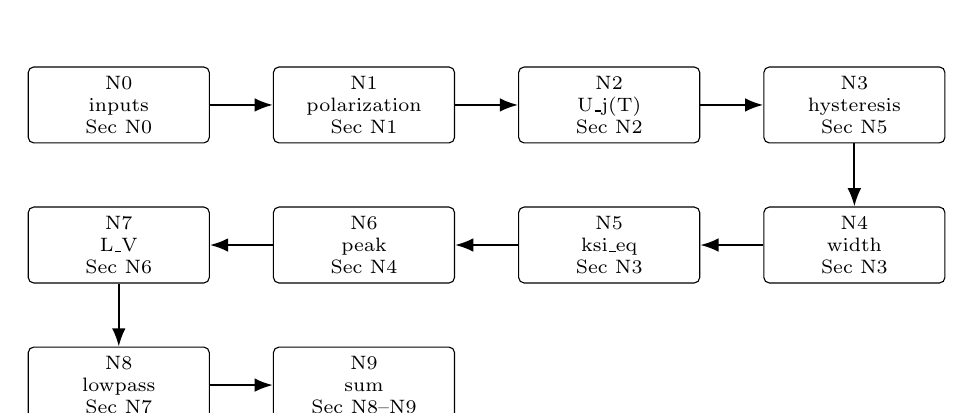
\begin{tikzpicture}[node distance=8mm, box/.style={draw,rounded corners=2pt,minimum width=23mm,minimum height=7mm,align=center,font=\scriptsize}, arr/.style={-Latex,thick}]
\node[box] (n0) {N0\\inputs\\Sec N0};
\node[box,right=of n0] (n1) {N1\\polarization\\Sec N1};
\node[box,right=of n1] (n2) {N2\\U\_j(T)\\Sec N2};
\node[box,right=of n2] (n3) {N3\\hysteresis\\Sec N5};
\node[box,below=of n3] (n4) {N4\\width\\Sec N3};
\node[box,left=of n4] (n5) {N5\\ksi\_eq\\Sec N3};
\node[box,left=of n5] (n6) {N6\\peak\\Sec N4};
\node[box,left=of n6] (n7) {N7\\L\_V\\Sec N6};
\node[box,below=of n7] (n8) {N8\\lowpass\\Sec N7};
\node[box,right=of n8] (n9) {N9\\sum\\Sec N8--N9};
\draw[arr] (n0) -- (n1);
\draw[arr] (n1) -- (n2);
\draw[arr] (n2) -- (n3);
\draw[arr] (n3) -- (n4);
\draw[arr] (n4) -- (n5);
\draw[arr] (n5) -- (n6);
\draw[arr] (n6) -- (n7);
\draw[arr] (n7) -- (n8);
\draw[arr] (n8) -- (n9);
\end{tikzpicture}
\caption{v11 계산 흐름을 절 순서로 옮긴 그림이다. 각 노드는 코드 노드와 본문 절 번호를 함께 표시하므로 그림에서 본문으로 바로 이동할 수 있다. 그림 내부 텍스트는 English ASCII 라벨만 사용했다.}
\label{fig:spine}
\end{figure}

\tableofcontents
\newpage
\setcounter{section}{-1}

% ====================================================================
\section{실험조건과 입력 격자}\label{sec:n0}
% ====================================================================
식~\eqref{eq:entry} 의 목적은 측정 격자 $V_{\app}$ 를 내부 계산 격자에 올리는 것이다. 이 절은 실험 조건을 모델 입력으로 닫고, 다음 절의 분극 보정이 작동할 전위 배열을 준비한다.

코드의 핵심 입력은
\begin{equation}
\{V_{\app},\,T,\,I_{\abs},\,Q_{\cellc},\,s\}
\quad\text{with}\quad s\mapsto\sigma_d=+1\ \text{if}\ s\ge0,\quad \sigma_d=-1\ \text{if}\ s<0.
\label{eq:n0input}
\end{equation}
$T$ 는 스칼라 등온 입력이거나 $V_{\app}$ 와 같은 길이의 배열이다. 배열이면 뒤에서 작업 격자에 보간되고, 스칼라이면 같은 값으로 채운다.

셀 정규화 진행량은 첫 사용부터
\begin{equation}
q=\frac{Q}{Q_{\cellc}},\qquad
\dot q=\frac{I_{\abs}}{Q_{\cellc}}
\label{eq:qdef}
\end{equation}
로 둔다. 따라서 $q$ 는 무차원 누적 전하이고, $Q_{\cellc}$ 는 C-rate 와 $L_q$ 환산에 공통으로 들어가는 셀 용량이다. 본문에서 $|\dd V/\dd q|_{q_a}$ 를 쓸 때의 $q$ 는 항상 식~\eqref{eq:qdef} 의 정규화 변수다.

분극 보정 뒤의 $V_n$ 가 정해지면 작업 격자는 그 범위를 양쪽으로 확장한다.
\begin{align}
v_{\lo}&=\min V_n,\qquad v_{\hi}=\max V_n,\qquad
v_{\mathrm{span}}=\max(v_{\hi}-v_{\lo},\texttt{v\_span\_floor}),\label{eq:vspan}\\
n_{\work}&=\max(\texttt{n\_work\_min},\,2\,\mathrm{size}(V_n)),\label{eq:nwork}\\
V_{\work}&=\mathrm{linspace}\!\left(v_{\lo}-\texttt{grid\_pad\_lo}\,v_{\mathrm{span}},
v_{\hi}+\texttt{grid\_pad\_hi}\,v_{\mathrm{span}},n_{\work}\right),\label{eq:vwork}\\
\texttt{grid\_step}&=V_{\work}[1]-V_{\work}[0].\label{eq:gridstep}
\end{align}
배경은 같은 격자 위에서 먼저 놓인다.
\begin{equation}
\texttt{dqdv\_work}=
\begin{cases}
C_{\bg}(V_{\work}),& C_{\bg}\ \text{가 callable 일 때},\\
C_{\bg}\,\bm 1,& C_{\bg}\ \text{가 상수일 때}.
\end{cases}
\label{eq:cbgwork}
\end{equation}

생성자에서 닫히는 비자명 기본값은 다음과 같다. 전이 사전의 같은 이름 key 가 있으면 전이별 override 가 우선한다.
\begin{center}
\renewcommand{\arraystretch}{1.18}
\begin{tabular}{lll}
\toprule
identifier & default & role\\
\midrule
\texttt{x} & 0.5 & fallback \texttt{chi}; transition-state fraction\\
\texttt{Rn} & 0.0 & series resistance for Eq.~\eqref{eq:polar}\\
\texttt{Cbg} & 0.0 & constant or callable background\\
\texttt{chi} & \texttt{None}$\to$\texttt{x} & global charge-transfer split\\
\texttt{chi\_split} & \texttt{func\_chi\_d} & discharge $\chi$, charge $1-\chi$\\
\texttt{use\_dH\_eff} & \texttt{True} & apply $\Delta H_a^{\eff}=\Delta H_a-\chi_d\Omega$\\
\texttt{use\_w\_eff} & \texttt{False} & keep direct \texttt{w}/\texttt{n} width unless enabled\\
\texttt{z\_cut} & 4.357 & cutoff affinity multiplier\\
\texttt{A\_cap\_RT} & 4.0 & cap $A\le4RT$\\
\texttt{w\_eff\_floor\_frac} & 0.05 & floor for $w^{\eff}$\\
\texttt{grid\_pad\_lo}, \texttt{grid\_pad\_hi} & 0.15, 0.15 & work-grid voltage padding\\
\texttt{n\_work\_min} & 2048 & minimum work-grid length\\
\texttt{min\_lag\_grid\_steps} & 2.0 & sub-grid tail threshold\\
\texttt{v\_span\_floor} & $10^{-6}$ & minimum span used for padding\\
\texttt{seed\_T}, \texttt{seed\_I}, \texttt{seed\_Q\_cell} & 298.15, 0.1, 1.0 & representative seed $L_V$ condition\\
\bottomrule
\end{tabular}
\end{center}
이제 외부 관측 전위와 내부 열역학 전위를 구분할 준비가 끝났다. 다음 절은 이 둘을 잇는 유일한 코드식인 분극 보정을 쓴다.

% ====================================================================
\section{분극 분해}\label{sec:n1}
% ====================================================================
N0 의 $V_{\app}$ 는 측정 전위다. 전이 중심과 logistic 이 읽는 전위는 내부 음극 전위 $V_n$ 이므로, 코드는 첫 물리식으로 분극을 제거한다.

\begin{equation}
\boxed{\;V_n=V_{\app}-\sigma_d\,I_{\abs}\,R_n\;.}
\label{eq:polar}
\end{equation}
방전에서는 $\sigma_d=+1$ 이므로 $V_n=V_{\app}-I_{\abs}R_n$ 이다. 방전은 흑연 음극의 delithiation/oxidation 이므로 관측 전위는 평형 전위보다 높다. 즉 $\eta=V_{\app}-V_{\eq}>0$ 이고, 코드의 $V_n$ 은 $V_{\app}$ 에서 양의 anodic overpotential 을 제거한 내부 전위다. 충전에서는 $\sigma_d=-1$ 이므로 $V_n=V_{\app}+I_{\abs}R_n$ 이며, 관측 전위가 평형 전위보다 낮은 cathodic branch 를 되돌린다. 이 부호 하나가 관측축과 열역학축을 분리하고, 이후 모든 전이 계산은 $V_{\work}$ 위의 내부 전위로 진행된다.

\begin{figure}[t]
\centering
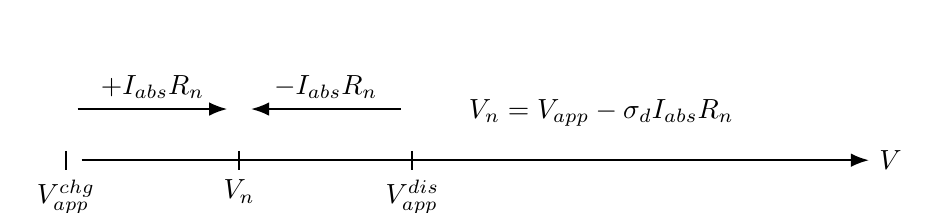
\begin{tikzpicture}[x=1.0cm,y=1.0cm, arr/.style={-Latex,thick}]
\draw[arr] (0,0) -- (10,0) node[right] {$V$};
\draw[thick] (2,0.12) -- (2,-0.12) node[below] {$V_n$};
\draw[thick] (4.2,0.12) -- (4.2,-0.12) node[below] {$V_{app}^{dis}$};
\draw[thick] (-0.2,0.12) -- (-0.2,-0.12) node[below] {$V_{app}^{chg}$};
\draw[arr] (4.05,0.65) -- (2.15,0.65) node[midway,above] {$-I_{abs}R_n$};
\draw[arr] (-0.05,0.65) -- (1.85,0.65) node[midway,above] {$+I_{abs}R_n$};
\node at (6.6,0.6) {$V_n=V_{app}-\sigma_d I_{abs}R_n$};
\end{tikzpicture}
\caption{분극 보정의 부호를 새로 그린 도식이다. 방전과 충전 모두 식~\eqref{eq:polar} 하나로 내부 전위 $V_n$ 에 도달한다.}
\label{fig:polar}
\end{figure}

분극 보정이 끝나면 다음 계산은 전이별 반복문으로 들어간다. 첫 전이별 양은 평형 중심 $U_j(T)$ 이며, 이 값이 logistic 중심과 hysteresis 분기 중심의 기준점이 된다.

% ====================================================================
\section{평형 중심 $U_j(T)$}\label{sec:n2}
% ====================================================================
N1 이 관측축을 내부축으로 옮겼다면, N2 는 전이 $j$ 의 기준 전위를 온도에서 계산한다. 코드에서 전이 사전이 \texttt{dH\_rxn} 과 \texttt{dS\_rxn} 을 갖고 있으면 \texttt{func\_U\_j} 가 우선한다.

\begin{equation}
\boxed{\;U_j(T)=\frac{-\Delta H_{\mathrm{rxn},j}+T\,\Delta S_{\mathrm{rxn},j}}{F}\;.}
\label{eq:Uj}
\end{equation}
전이 사전에 열역학 쌍이 없으면 코드의 fallback 은 직접 입력된 \texttt{U} 다.
\begin{equation}
U_j=
\begin{cases}
\texttt{func\_U\_j}(T,\texttt{dH\_rxn},\texttt{dS\_rxn}),& \texttt{dH\_rxn},\texttt{dS\_rxn}\ \text{존재},\\
\texttt{U},&\text{그 밖의 경우}.
\end{cases}
\label{eq:Udispatch}
\end{equation}
식~\eqref{eq:Uj} 의 부호는 $\Delta G=-FU$ 를 코드 형태로 쓴 것이다. $\Delta H_{\mathrm{rxn}}<0$ 이고 $\Delta S_{\mathrm{rxn}}$ 가 작으면 $-\Delta H_{\mathrm{rxn}}/F$ 가 양의 전위를 만든다.

v11 의 기본 staging 초기값은 피팅 시작점이다.
\begin{center}
\renewcommand{\arraystretch}{1.25}
\begin{tabular}{lrrrrrrrrr}
\toprule
transition & \texttt{U} & \texttt{w} & \texttt{Q} & \texttt{Omega} & \texttt{dH\_rxn} & \texttt{dS\_rxn} & \texttt{dH\_a} & \texttt{dVdq\_qa} & \texttt{dS\_a}\\
\midrule
stage $4\to3$ & 0.210 & 0.020 & 0.10 & 6000 & -11700 & +29 & 48000 & 0.30 & 0\\
stage $3\to2L$ & 0.140 & 0.016 & 0.12 & 8000 & -13500 & 0 & 46000 & 0.30 & 0\\
stage $2L\to2$ & 0.120 & 0.014 & 0.25 & 10000 & -13100 & -5 & 44000 & 0.30 & 0\\
stage $2\to1$ & 0.085 & 0.012 & 0.50 & 13000 & -13000 & -16 & 40000 & 0.30 & 0\\
\bottomrule
\end{tabular}
\end{center}
여기서 \texttt{dH\_a}, \texttt{dVdq\_qa}, \texttt{dS\_a} 는 N7 동역학 branch 의 초기값이다. 모든 값은 v11 의 \texttt{GRAPHITE\_STAGING\_LIT} 에 들어 있는 피팅 시작점이며, 신뢰 고정값이 아니라 전이별 override 대상이다.
평형 중심은 아직 방향을 모른다. 방향별 중심 이동은 hysteresis 분기가 있을 때만 생기며, 그 전에 폭과 점유율을 계산할 수 있도록 다음 절에서 logistic 의 폭을 닫는다.

% ====================================================================
\section{폭과 평형 점유율}\label{sec:n3}
% ====================================================================
N2 의 $U_j(T)$ 는 중심이고, N3 의 폭 $w$ 는 그 중심 주변에서 점유율이 얼마나 빠르게 바뀌는지를 정한다. 평형 점유율은 두 상태의 chemical potential equality 에서 나온다. 한 전이 안에서 빈 자리와 채워진 자리의 혼합항을
\begin{equation}
\mu_{\mathrm{occ}}-\mu_{\mathrm{vac}}
=\Delta\mu_j^0-n_jF\sigma_d V_n
+RT\ln\frac{\xi_j}{1-\xi_j}
\label{eq:mueqraw}
\end{equation}
로 쓰면, 평형은 $\mu_{\mathrm{occ}}=\mu_{\mathrm{vac}}$ 이다. 기준 전위 $U_j$ 는 $\Delta\mu_j^0=n_jF\sigma_d U_j$ 를 만족하는 중심이므로
\begin{equation}
\ln\frac{\xi_{\eq,j}}{1-\xi_{\eq,j}}
=\frac{\sigma_d(V_n-U_j)}{n_jRT/F}
=\frac{\sigma_d(V_n-U_j)}{w_j}
\label{eq:logitsolve}
\end{equation}
가 된다. 이는 Fermi--Dirac 점유율 $f=[1+\exp((\epsilon-\mu)/k_BT)]^{-1}$ 과 같은 algebra 이며, 전위가 site energy 와 electrochemical potential 의 차이를 대신한다. 따라서 $\xi_{\eq}\to0$ 은 $z\to-\infty$, $\xi_{\eq}\to1$ 은 $z\to+\infty$ 로 고정된다.

코드는 먼저 \texttt{n} 또는 \texttt{w} 에서 다중도 $n_j$ 를 얻는다.

\begin{equation}
n_j(T)=
\begin{cases}
\texttt{n},&\texttt{n}\ \text{이 주어질 때},\\
\texttt{w}\,F/(RT),&\texttt{w}\ \text{가 주어질 때},\\
1,&\text{그 밖의 경우}.
\end{cases}
\label{eq:nfactor}
\end{equation}
기본 폭은 \texttt{func\_w} 이다.
\begin{equation}
\boxed{\;w_j(T)=\frac{n_jRT}{F}\;.}
\label{eq:w}
\end{equation}
\texttt{use\_w\_eff} 가 켜지고 \texttt{Omega} 가 있으며 직접 \texttt{w} 가 없으면 코드는 유효 폭을 쓴다.
\begin{equation}
w_j^{\eff}(T)=
\max\!\left[
\frac{RT}{F}\left(1-\frac{\Omega_j}{2RT}\right),
\texttt{w\_eff\_floor\_frac}\frac{RT}{F}
\right].
\label{eq:weffcode}
\end{equation}
폭이 정해지면 평형 점유율은 코드의 \texttt{func\_ksi\_eq} 그대로다.
\begin{equation}
z_j=\frac{\sigma_d\left(V_{\work}-\texttt{center}_j\right)}{w_j},
\qquad
\boxed{\;\xi_{\eq,j}=\frac{1}{1+\exp(-z_j)}\;.}
\label{eq:ksieq}
\end{equation}
큰 $|z|$ 에서 overflow 를 피하려고 구현은 양수와 음수 branch 를 나누지만, 수식의 내용은 식~\eqref{eq:ksieq} 하나다. 방전에서는 $\sigma_d=+1$ 이므로 $V$ 가 오르면 $\xi_{\eq}$ 가 오른다. 충전에서는 $\sigma_d=-1$ 이므로 $V$ 가 내려가는 진행 방향에서 $\xi_{\eq}$ 가 오른다.

\begin{figure}[t]
\centering
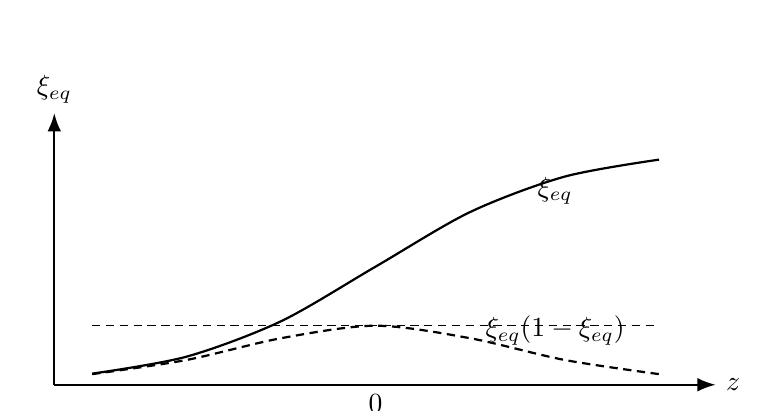
\begin{tikzpicture}[x=1.2cm,y=3.0cm]
\draw[-Latex,thick] (-3.4,0) -- (3.6,0) node[right] {$z$};
\draw[-Latex,thick] (-3.4,0) -- (-3.4,1.15) node[above] {$\xi_{eq}$};
\draw[thick] plot[smooth] coordinates {(-3,0.047) (-2,0.119) (-1,0.269) (0,0.5) (1,0.731) (2,0.881) (3,0.953)};
\draw[densely dashed] (-3,0.25) -- (3,0.25);
\draw[thick,densely dashed] plot[smooth] coordinates {(-3,0.045) (-2,0.105) (-1,0.197) (0,0.25) (1,0.197) (2,0.105) (3,0.045)};
\node at (1.9,0.82) {$\xi_{eq}$};
\node at (1.9,0.23) {$\xi_{eq}(1-\xi_{eq})$};
\node[below] at (0,0) {$0$};
\end{tikzpicture}
\caption{식~\eqref{eq:ksieq} 의 logistic 과 식~\eqref{eq:dxidv} 의 종 모양 인자를 새로 그렸다. 코드의 방향 부호는 $z$ 의 정의 안에 들어간다.}
\label{fig:logistic}
\end{figure}

점유율은 peak 가 아니라 상태다. 다음 절은 이 상태의 전위 미분을 취해 평형 ICA peak 를 얻는다.

% ====================================================================
\section{평형 peak 위치와 높이}\label{sec:n4}
% ====================================================================
N3 이 $\xi_{\eq,j}$ 를 닫았으므로, 평형 peak 는 그 전위 미분이다. 코드의 저율 branch 와 \texttt{equilibrium()} 은 같은 식을 사용한다.

\begin{align}
\frac{\dd\xi_{\eq,j}}{\dd V}
&=\frac{\dd\xi_{\eq,j}}{\dd z_j}\frac{\dd z_j}{\dd V}
=\xi_{\eq,j}(1-\xi_{\eq,j})\frac{\sigma_d}{w_j},\label{eq:dxidv}\\
\left|\frac{\dd\xi_{\eq,j}}{\dd V}\right|
&=\frac{\xi_{\eq,j}(1-\xi_{\eq,j})}{w_j}.\label{eq:absdxidv}
\end{align}
따라서 코드의 평형 peak shape 는 방향과 무관한 양수다.
\begin{equation}
\boxed{\;\texttt{peak\_shape}_{j,\eqm}=
\frac{\xi_{\eq,j}(1-\xi_{\eq,j})}{w_j}\;.}
\label{eq:eqpeakshape}
\end{equation}
\texttt{equilibrium(V\_n,T)} 는 hysteresis 와 tail 을 넣지 않고
\begin{equation}
\boxed{\;\texttt{equilibrium}(V_n,T)=
C_{\bg}+\sum_j Q_j\,\frac{\xi_{\eq,j}(1-\xi_{\eq,j})}{w_j}\;.}
\label{eq:equilibrium}
\end{equation}
전이 하나의 중심에서 $\xi_{\eq}=1/2$ 이므로 순높이는 $Q_j/(4w_j)$ 이고 중심은 hysteresis 가 없을 때 $U_j$ 다.

평형 peak 는 모든 방향과 전류 효과의 기준선이다. 다음 절은 그 중심을 방향별로 밀어 충방전 hysteresis 를 넣는다.

% ====================================================================
\section{히스테리시스 분기}\label{sec:n5}
% ====================================================================
N4 의 peak 중심은 단일 $U_j$ 였다. 상호작용이 충분히 크고 \texttt{gamma} 가 켜진 전이는 v11 에서 방향별 중심 \texttt{center} 로 갈라진다.

먼저 \texttt{func\_dU\_hys} 는 spinodal 상한 gap 을 계산한다. 정규용액 double-well 의 무차원 점유 free energy 를
\begin{equation}
g(\xi)=RT\{\xi\ln\xi+(1-\xi)\ln(1-\xi)\}
\,+\Omega\,\xi(1-\xi)-F U\,\xi
\label{eq:doublewell}
\end{equation}
로 쓰면, 내부 chemical potential 의 혼합 부분은
\begin{equation}
\mu_{\mathrm{mix}}(\xi)=RT\ln\frac{\xi}{1-\xi}+\Omega(1-2\xi)
\label{eq:mumix}
\end{equation}
이다. Spinodal 은 $g''(\xi)=0$ 이므로
\begin{equation}
\frac{RT}{\xi(1-\xi)}-2\Omega=0,\qquad
\xi_\pm=\frac{1\pm u}{2},\qquad
u=\sqrt{1-\frac{2RT}{\Omega}}.
\label{eq:spinodalsolve}
\end{equation}
$\Omega\le2RT$ 에서는 실수 spinodal 이 없으므로 double-well 분리가 사라진다. $\Omega>2RT$ 에서 두 spinodal 의 voltage separation 은
\begin{equation}
\Delta U_{\hys}
=\frac{\mu_{\mathrm{mix}}(\xi_-)-\mu_{\mathrm{mix}}(\xi_+)}{F}
=\frac{2}{F}\left[\Omega u-2RT\,\operatorname{artanh}u\right]
\label{eq:dUhysderive}
\end{equation}
이며, 이것이 코드의 gap 이다.
\begin{equation}
\Delta U_{\hys,j}(T,\Omega_j)=
\begin{cases}
0,&\Omega_j\le2RT,\\[3pt]
\dfrac{2}{F}\left[\Omega_j u_j-2RT\,\operatorname{artanh}u_j\right],
&\Omega_j>2RT,
\end{cases}
\qquad
u_j=\sqrt{1-\frac{2RT}{\Omega_j}}.
\label{eq:dUhys}
\end{equation}
이 값은 항상 음수가 아닌 gap 이다. \texttt{func\_U\_branch} 는 이 gap 의 절반을 방향 부호로 더한다.
\begin{equation}
\boxed{\;U_j^{d}=U_j+\frac12\,\sigma_d\,h_{\eta,j}\,\gamma_j\,\Delta U_{\hys,j}\;.}
\label{eq:Ubranch}
\end{equation}
반복문 안의 구현은 배열 $U_j(T_{\work})$ 에 대표 온도 $T_{\rep}$ 로 계산한 상수 shift 를 더한다.
\begin{equation}
\texttt{hys\_shift}_j=
\texttt{func\_U\_branch}(T_{\rep},0,\Omega_j,\gamma_j,\sigma_d,h_{\eta,j}),
\qquad
\texttt{center}_j=U_j+\texttt{hys\_shift}_j.
\label{eq:center}
\end{equation}
$\gamma_j=0$ 이거나 $\Omega_j=0$ 이면 \texttt{center}$=U_j$ 로 돌아간다. 방전은 $\sigma_d=+1$ 이므로 중심이 위로 움직이고, 충전은 $\sigma_d=-1$ 이므로 중심이 아래로 움직인다.

\begin{figure}[t]
\centering
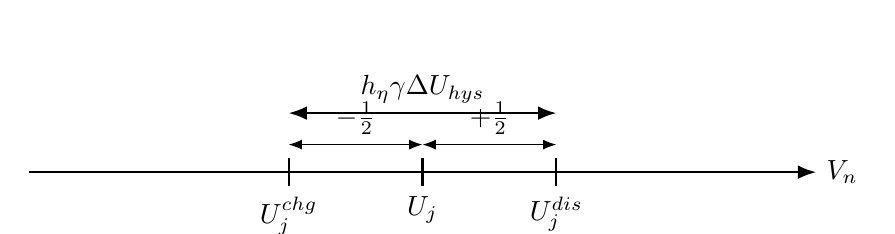
\begin{tikzpicture}[x=1.0cm,y=1.0cm]
\draw[-Latex,thick] (0,0) -- (10,0) node[right] {$V_n$};
\draw[thick] (5,0.18) -- (5,-0.18) node[below] {$U_j$};
\draw[thick] (6.7,0.18) -- (6.7,-0.18) node[below] {$U_j^{dis}$};
\draw[thick] (3.3,0.18) -- (3.3,-0.18) node[below] {$U_j^{chg}$};
\draw[Latex-Latex,thick] (3.3,0.75) -- (6.7,0.75) node[midway,above] {$h_\eta\gamma\Delta U_{hys}$};
\draw[Latex-Latex] (5,0.35) -- (6.7,0.35) node[midway,above] {$+\frac12$};
\draw[Latex-Latex] (3.3,0.35) -- (5,0.35) node[midway,above] {$-\frac12$};
\end{tikzpicture}
\caption{분기 중심 식~\eqref{eq:Ubranch} 의 방향 부호를 새로 그린 도식이다. 방전과 충전 중심은 $U_j$ 를 사이에 두고 반대쪽으로 이동한다.}
\label{fig:hys}
\end{figure}

분기 중심은 logistic 의 중심만 바꾼다. 다음 절은 같은 중심을 갖는 $\xi_{\eq}$ 가 전류와 속도 때문에 얼마나 늦게 따라오는지를 $L_q$ 와 $L_V$ 로 계산한다.

% ====================================================================
\section{동역학 꼬리 길이}\label{sec:n6}
% ====================================================================
N5 가 방향별 중심을 만들었으므로, N6 은 전이별 지연 길이 \texttt{lag\_len\_V} 를 계산한다. 직접 \texttt{L\_V} 가 주어지면 코드가 그것을 사용하고, 아니면 Eyring--Butler--Volmer 형태의 \texttt{func\_L\_q} 를 호출한다.

직접 지정 branch 는
\begin{equation}
\texttt{lag\_len\_V}=L_V\qquad(\texttt{L\_V}\ \text{직접 지정})
\label{eq:LVoverride}
\end{equation}
이다. 동역학 branch 는 전압축 tail 이 아니라 먼저 $q$ 축 relaxation length 를 만든다. 진행량 $q=Q/Q_{\cellc}$ 에서 국소 완화식을
\begin{equation}
\frac{\dd \xi}{\dd t}=\frac{\xi_{\eq}-\xi}{\tau_j},
\qquad
\frac{\dd q}{\dd t}=\frac{I_{\abs}}{Q_{\cellc}}
\label{eq:tautokuq}
\end{equation}
로 쓰면, 같은 식은 $q$ 축에서
\begin{equation}
\frac{\dd \xi}{\dd q}=\frac{\xi_{\eq}-\xi}{L_{q,j}},
\qquad
L_{q,j}=\frac{I_{\abs}}{Q_{\cellc}}\tau_j
\label{eq:Lqmotivation}
\end{equation}
가 된다. 연속형 기억 해는 진행 방향 coordinate $r\ge0$ 에 대해
\begin{equation}
\xi_{\mathrm{lag}}(q)=\int_{0}^{\infty}\frac{1}{L_{q,j}}
\exp\!\left(-\frac{r}{L_{q,j}}\right)\xi_{\eq}(q-r)\,\dd r
\label{eq:Lqintegral}
\end{equation}
이고, 균일 격자에서는 같은 kernel 이 뒤의 식~\eqref{eq:lowpass} 의 지수 재귀로 구현된다.

동역학 branch 에서는 먼저 cutoff affinity 를 만든다.
\begin{equation}
A_j=\min\!\left(\texttt{z\_cut}\,|n_j|RT,\ \texttt{A\_cap\_RT}\,RT\right).
\label{eq:Acut}
\end{equation}
방향별 전달계수는 코드의 \texttt{func\_chi\_d} 이다.
\begin{equation}
\boxed{\;\chi_d=
\begin{cases}
\chi,&\sigma_d\ge0,\\
1-\chi,&\sigma_d<0.
\end{cases}\;}
\label{eq:chid}
\end{equation}
상호작용 보강이 켜져 있으면 활성화 엔탈피는 \texttt{func\_dH\_a\_eff} 로 바뀐다.
\begin{equation}
\boxed{\;\Delta H_{a,j}^{\eff}=\Delta H_{a,j}-\chi_d\,\Omega_j\;.}
\label{eq:dHeff}
\end{equation}
이제 \texttt{func\_L\_q} 의 로그식이 그대로 나온다.
\begin{align}
T_{\mathrm{attempt}}&=\frac{I_{\abs}}{Q_{\cellc}}\frac{h}{k_B},\label{eq:Tattempt}\\
\Delta G_{a,j}^{\eff}&=\Delta H_{a,j}^{\eff}-T\Delta S_{a,j},\label{eq:dGeff}\\
\ln L_{q,j}
&=\ln\frac{T_{\mathrm{attempt}}}{T}
-\ln\!\left(1+e^{-A_j/(RT)}\right)
+\frac{\Delta G_{a,j}^{\eff}}{RT}
-\frac{\chi_d A_j}{RT},\label{eq:lnLq}\\
\boxed{\;\begin{aligned}
L_{q,j}
&=\frac{I_{\abs}h}{Q_{\cellc}k_BT}\,
\exp\!\left[\frac{\Delta G_{a,j}^{\eff}-\chi_d A_j}{RT}\right]\\
&\quad{}\times\left(1+\exp[-A_j/(RT)]\right)^{-1}\;.
\end{aligned}}
\label{eq:Lq}
\end{align}
식~\eqref{eq:Lq} 는 식~\eqref{eq:Lqmotivation} 의 $\tau_j$ 에 Eyring prefactor $h/(k_BT)$ 와 Butler--Volmer barrier factor 를 넣은 것이다. $-\chi_d A_j/(RT)$ 는 방전에서는 $\chi$, 충전에서는 $1-\chi$ 가 곱해지는 방향별 장벽 저하 항이다.

전압축 길이는 cutoff 위치의 OCV 기울기 크기로 환산한다.
\begin{equation}
\boxed{\;\begin{aligned}
L_{V,j}
&=\left|\frac{\dd V}{\dd q}\right|_{q_a}\,L_{q,j}\\
&=|\texttt{dVdq\_qa}|\,L_{q,j}\;.
\end{aligned}}
\label{eq:LV}
\end{equation}
v11 구현에서 $A_j$ 는 전이별 cutoff parameter 로 한 번 정해지는 상수다. \texttt{\_resolve\_lag\_length} 는 대표 온도와 대표 $n_j$ 에서 $A_j=\min(\texttt{z\_cut}|n_j|RT,\texttt{A\_cap\_RT}RT)$ 를 만들고, 같은 전이 안의 모든 $V_{\work}$ 점에 같은 $L_{q,j}$ 를 쓴다. 따라서 plateau 내부에서는
\begin{equation}
\frac{\partial \ln L_{q,j}}{\partial V}=0
\qquad\text{within one v11 transition plateau.}
\label{eq:Lqflat}
\end{equation}
전위가 오르면 장벽이 낮아지고 꼬리가 짧아진다는 $\dd U/\dd V<0$ 또는 graphite OCV slope 직관은 식~\eqref{eq:Lq} 의 물리적 동기다. 하지만 v11 의 계산식은 그 미분을 실시간으로 평가하지 않으며, $L_q$ 는 전이별 piecewise-flat 상수로 들어간다.

꼬리 길이가 격자보다 너무 작으면 코드는 평형 peak 로 환원한다.
\begin{equation}
L_{V,j}<\texttt{min\_lag\_grid\_steps}\cdot\texttt{grid\_step}
\quad\Longrightarrow\quad
\texttt{peak\_shape}_j=\frac{\xi_{\eq,j}(1-\xi_{\eq,j})}{w_j}.
\label{eq:lagthreshold}
\end{equation}
그렇지 않으면 다음 절의 인과 기억 필터가 켜진다.

% ====================================================================
\section{인과 기억 꼬리와 충전 격자 역전}\label{sec:n7}
% ====================================================================
N6 의 $L_{V,j}$ 가 충분히 크면, v11 은 $\xi_{\eq}$ 자체를 미분하지 않는다. 진행 방향의 과거를 지수 기억으로 low-pass 한 \texttt{occ\_lagged} 를 만든 뒤, 현재 평형 목표와 지연 점유의 차이를 $L_V$ 로 나눈다.

감쇠율은
\begin{equation}
a_j=\exp\!\left(-\frac{\texttt{grid\_step}}{L_{V,j}}\right)
\label{eq:decay}
\end{equation}
이고, \texttt{\_causal\_lowpass} 의 재귀형은
\begin{equation}
y_0=x_0,\qquad
y_i=a_jy_{i-1}+(1-a_j)x_i\quad(i\ge1).
\label{eq:lowpass}
\end{equation}
방전은 $V_{\work}$ 의 오름차순이 진행 방향과 같으므로 그대로 필터링한다.
\begin{equation}
\sigma_d\ge0:\qquad
\texttt{occ\_lagged}=\mathcal L_{L_V}(\xi_{\eq}).
\label{eq:dislowpass}
\end{equation}
충전은 진행 방향이 $V$ 감소 방향이므로 격자를 반드시 뒤집는다.
\begin{equation}
\sigma_d<0:\qquad
\texttt{occ\_lagged}=
\left[\mathcal L_{L_V}\!\left(\xi_{\eq}[::-1]\right)\right][::-1].
\label{eq:chglowpass}
\end{equation}
이 역전이 없으면 충전 꼬리가 미래를 보는 비인과 필터가 되고, 충전 $dQ/dV$ 의 양수 거울상이 깨진다. v11 의 tail peak 는 다음 한 줄이다.
\begin{equation}
\boxed{\;\texttt{peak\_shape}_j=
\frac{\xi_{\eq,j}-\texttt{occ\_lagged}_j}{L_{V,j}}\;.}
\label{eq:tailpeak}
\end{equation}
$L_V$ 가 작아질수록 low-pass 의 지연은 사라지고, 식~\eqref{eq:lagthreshold} 의 평형 peak 로 돌아간다.

\begin{figure}[t]
\centering
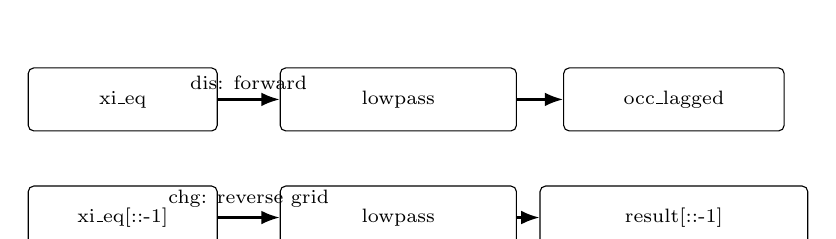
\begin{tikzpicture}[x=1.0cm,y=1.0cm, arr/.style={-Latex,thick}]
\node[draw,rounded corners=2pt,minimum width=24mm,minimum height=8mm,font=\scriptsize] (x) at (0,0) {xi\_eq};
\node[draw,rounded corners=2pt,minimum width=30mm,minimum height=8mm,font=\scriptsize] (f) at (3.5,0) {lowpass};
\node[draw,rounded corners=2pt,minimum width=28mm,minimum height=8mm,font=\scriptsize] (y) at (7,0) {occ\_lagged};
\draw[arr] (x) -- node[above,font=\scriptsize] {dis: forward} (f);
\draw[arr] (f) -- (y);
\node[draw,rounded corners=2pt,minimum width=24mm,minimum height=8mm,font=\scriptsize] (xr) at (0,-1.5) {xi\_eq[::-1]};
\node[draw,rounded corners=2pt,minimum width=30mm,minimum height=8mm,font=\scriptsize] (fr) at (3.5,-1.5) {lowpass};
\node[draw,rounded corners=2pt,minimum width=34mm,minimum height=8mm,font=\scriptsize] (yr) at (7,-1.5) {result[::-1]};
\draw[arr] (xr) -- node[above,font=\scriptsize] {chg: reverse grid} (fr);
\draw[arr] (fr) -- (yr);
\end{tikzpicture}
\caption{인과 기억 필터를 새로 그린 도식이다. 충전에서는 코드의 \texttt{[::-1]} 역전과 재역전이 진행 방향의 과거를 보장한다.}
\label{fig:lowpass}
\end{figure}

이제 각 전이는 양수 peak shape 를 갖는다. 마지막 절은 전이 용량 $Q_j$ 를 곱해 누적하고, 작업 격자에서 원래 $V_n$ 배열로 되돌린다.

% ====================================================================
\section{전이별 합산}\label{sec:n8}
% ====================================================================
N7 의 \texttt{peak\_shape} 는 전이 하나의 단위 전하 모양이다. v11 은 각 전이 용량 \texttt{Q} 를 곱해 작업 배열에 더한다.

\begin{equation}
\texttt{dqdv\_work}
=C_{\bg}(V_{\work},T)+
\sum_{j=1}^{N_p}Q_j\,\texttt{peak\_shape}_j.
\label{eq:worksum}
\end{equation}
식~\eqref{eq:worksum} 의 \texttt{peak\_shape} 는 두 branch 중 하나다.
\begin{equation}
\texttt{peak\_shape}_j=
\begin{cases}
\xi_{\eq,j}(1-\xi_{\eq,j})/w_j,&
L_{V,j}<\texttt{min\_lag\_grid\_steps}\cdot\texttt{grid\_step},\\[5pt]
(\xi_{\eq,j}-\texttt{occ\_lagged}_j)/L_{V,j},&
\text{그 밖의 경우}.
\end{cases}
\label{eq:peakbranch}
\end{equation}
따라서 한 곡선의 폐형은 코드 branch 를 유지한 합산식으로 읽어야 한다.
\begin{equation}
\boxed{\;\frac{\dd Q}{\dd V}(V_{\work})=
C_{\bg}+\sum_j Q_j
\left[
\frac{\xi_{\eq,j}(1-\xi_{\eq,j})}{w_j}
\ \text{or}\
\frac{\xi_{\eq,j}-\texttt{occ\_lagged}_j}{L_{V,j}}
\right]\;.}
\label{eq:closedcode}
\end{equation}
여기서 ``or'' 는 수학적 자유 선택이 아니라 식~\eqref{eq:peakbranch} 의 코드 branch 다. 평형 branch 는 저율과 sub-grid 지연의 극한이고, 기억 branch 는 finite-rate tail 이다.

% ====================================================================
\section{역보간과 반환값}\label{sec:n9}
% ====================================================================
N8 의 합산은 확장 작업 격자 위에 있다. v11 의 마지막 일은 분극 보정으로 얻은 원래 $V_n$ 배열에 다시 보간하는 것이다.

\begin{equation}
\boxed{\;\texttt{dqdv\_out}=
\mathrm{interp}(V_n,V_{\work},\texttt{dqdv\_work})\;.}
\label{eq:interp}
\end{equation}
입력이 스칼라였으면 첫 원소를 스칼라로 반환하고, 배열이면 배열로 반환한다.
\begin{equation}
\texttt{return}=
\begin{cases}
\texttt{float(dqdv\_out[0])},&V_{\app}\ \text{스칼라 입력},\\
\texttt{dqdv\_out},&V_{\app}\ \text{배열 입력}.
\end{cases}
\label{eq:return}
\end{equation}
전체 사슬을 한 줄로 모으면
\begin{equation}
V_{\app}
\xrightarrow{\;V_n=V_{\app}-\sigma_d I_{\abs}R_n\;}
V_{\work}
\xrightarrow{\;\sum_j Q_j\,\texttt{peak\_shape}_j+C_{\bg}\;}
\texttt{dqdv\_work}
\xrightarrow{\;\mathrm{interp}\;}
\frac{\dd Q}{\dd V}(V_{\app}).
\label{eq:wholechain}
\end{equation}

\begin{figure}[t]
\centering
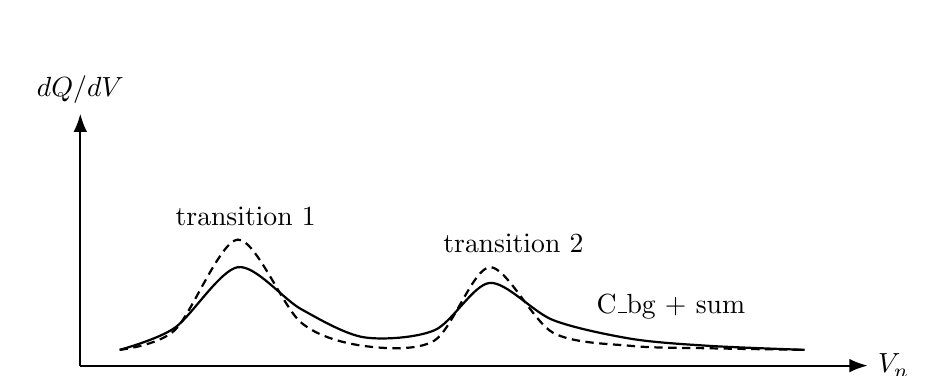
\begin{tikzpicture}[x=1.0cm,y=1.0cm]
\draw[-Latex,thick] (0,0) -- (10,0) node[right] {$V_n$};
\draw[-Latex,thick] (0,0) -- (0,3.2) node[above] {$dQ/dV$};
\draw[thick,densely dashed] plot[smooth] coordinates {(0.5,0.2) (1.2,0.45) (2.0,1.6) (2.8,0.55) (3.6,0.25) (4.5,0.32) (5.2,1.25) (6.0,0.42) (7.0,0.25) (8.0,0.22) (9.2,0.2)};
\draw[thick] plot[smooth] coordinates {(0.5,0.2) (1.2,0.48) (2.0,1.25) (2.8,0.72) (3.6,0.36) (4.5,0.45) (5.2,1.05) (6.0,0.58) (7.0,0.34) (8.0,0.25) (9.2,0.2)};
\node at (2.1,1.9) {transition 1};
\node at (5.5,1.55) {transition 2};
\node at (7.5,0.75) {C\_bg + sum};
\end{tikzpicture}
\caption{전이별 peak shape 를 더해 전체 $dQ/dV$ 를 만드는 새 그림이다. 파선은 평형 성분의 직관, 실선은 finite-rate tail 이 합쳐진 작업 격자 결과를 나타낸다.}
\label{fig:sum}
\end{figure}

\begin{keybox}
v11 의 Chapter 1 이 닫는 것은 식~\eqref{eq:wholechain} 이다. 부호는 네 위치에만 작용한다. 분극은 $-\sigma_d I_{\abs}R_n$, logistic 은 $\sigma_d(V-\texttt{center})/w$, 분기 중심은 $+\tfrac12\sigma_d h_\eta\gamma\Delta U_{\hys}$, 충전 tail 은 격자 역전이다. 이 네 곳이 맞으면 방전은 $V$ 상승 방향, 충전은 그 거울 방향에서 양의 $dQ/dV$ 로 반환된다.
\end{keybox}

\end{document}
